\documentclass[]{book}
\usepackage{lmodern}
\usepackage{amssymb,amsmath}
\usepackage{ifxetex,ifluatex}
\usepackage{fixltx2e} % provides \textsubscript
\ifnum 0\ifxetex 1\fi\ifluatex 1\fi=0 % if pdftex
  \usepackage[T1]{fontenc}
  \usepackage[utf8]{inputenc}
\else % if luatex or xelatex
  \ifxetex
    \usepackage{mathspec}
  \else
    \usepackage{fontspec}
  \fi
  \defaultfontfeatures{Ligatures=TeX,Scale=MatchLowercase}
\fi
% use upquote if available, for straight quotes in verbatim environments
\IfFileExists{upquote.sty}{\usepackage{upquote}}{}
% use microtype if available
\IfFileExists{microtype.sty}{%
\usepackage{microtype}
\UseMicrotypeSet[protrusion]{basicmath} % disable protrusion for tt fonts
}{}
\usepackage[margin=1in]{geometry}
\usepackage{hyperref}
\hypersetup{unicode=true,
            pdftitle={Predict Crypto Database Quick Start Guide},
            pdfauthor={Ricky Esclapon - riccardo.esclapon@colorado.edu},
            pdfborder={0 0 0},
            breaklinks=true}
\urlstyle{same}  % don't use monospace font for urls
\usepackage{natbib}
\bibliographystyle{apalike}
\usepackage{longtable,booktabs}
\usepackage{graphicx,grffile}
\makeatletter
\def\maxwidth{\ifdim\Gin@nat@width>\linewidth\linewidth\else\Gin@nat@width\fi}
\def\maxheight{\ifdim\Gin@nat@height>\textheight\textheight\else\Gin@nat@height\fi}
\makeatother
% Scale images if necessary, so that they will not overflow the page
% margins by default, and it is still possible to overwrite the defaults
% using explicit options in \includegraphics[width, height, ...]{}
\setkeys{Gin}{width=\maxwidth,height=\maxheight,keepaspectratio}
\IfFileExists{parskip.sty}{%
\usepackage{parskip}
}{% else
\setlength{\parindent}{0pt}
\setlength{\parskip}{6pt plus 2pt minus 1pt}
}
\setlength{\emergencystretch}{3em}  % prevent overfull lines
\providecommand{\tightlist}{%
  \setlength{\itemsep}{0pt}\setlength{\parskip}{0pt}}
\setcounter{secnumdepth}{5}
% Redefines (sub)paragraphs to behave more like sections
\ifx\paragraph\undefined\else
\let\oldparagraph\paragraph
\renewcommand{\paragraph}[1]{\oldparagraph{#1}\mbox{}}
\fi
\ifx\subparagraph\undefined\else
\let\oldsubparagraph\subparagraph
\renewcommand{\subparagraph}[1]{\oldsubparagraph{#1}\mbox{}}
\fi

%%% Use protect on footnotes to avoid problems with footnotes in titles
\let\rmarkdownfootnote\footnote%
\def\footnote{\protect\rmarkdownfootnote}

%%% Change title format to be more compact
\usepackage{titling}

% Create subtitle command for use in maketitle
\newcommand{\subtitle}[1]{
  \posttitle{
    \begin{center}\large#1\end{center}
    }
}

\setlength{\droptitle}{-2em}

  \title{Predict Crypto Database Quick Start Guide}
    \pretitle{\vspace{\droptitle}\centering\huge}
  \posttitle{\par}
    \author{Ricky Esclapon - \href{mailto:riccardo.esclapon@colorado.edu}{\nolinkurl{riccardo.esclapon@colorado.edu}}}
    \preauthor{\centering\large\emph}
  \postauthor{\par}
      \predate{\centering\large\emph}
  \postdate{\par}
    \date{2020-01-01}

\usepackage{booktabs}
\usepackage{amsthm}
\makeatletter
\def\thm@space@setup{%
  \thm@preskip=8pt plus 2pt minus 4pt
  \thm@postskip=\thm@preskip
}
\makeatother

\begin{document}
\maketitle

{
\setcounter{tocdepth}{1}
\tableofcontents
}
\hypertarget{overview}{%
\chapter{Overview}\label{overview}}

\href{https://predictcryptodb.com}{
\includegraphics{images/PredictCryptoLogo.PNG}}

This is a quick start guide for the \href{https://predictcryptodb.com}{Predict Crypto DataBase} which should provide the support you need to interact with the database and pull data. Everything you need to know will be outlined in this document and you can use the sidebar on the left to review the following sections:

\begin{enumerate}
\def\labelenumi{\arabic{enumi}.}
\item
  \protect\hyperlink{overview}{Overview-} This section.
\item
  \protect\hyperlink{interacting-with-the-db}{Interacting with the DB-} Instructions around accessing the \textbf{\emph{Metabase}} environment that will allow you to interact with the database, which is hosted on the website \href{https://predictcryptodb.com}{PredictCryptoDB.com}
\item
  \protect\hyperlink{useful-tables}{Useful Tables-} A review of some of the more useful/interesting tables you can find within the database and an overview of the best places to get started.
\item
  \protect\hyperlink{usage-guide}{Usage Guide-} This guide explores some of the functionality found within the website/Metabase environment.
\item
  \protect\hyperlink{documentation-usage}{Documentation Usage-} An overview of the documentation that is available through the Metabase environment and how to use it to answer questions you may have around where the data is sourced from as well as a complete data dictionary for every table.
\item
  \protect\hyperlink{additional-tips}{Additional Tips-} Some additional notes around using the environment to its full potential. This section goes over things like \protect\hyperlink{pulling-most-recent-data}{pulling the most recent data}, \protect\hyperlink{creating-dashboards}{creating dashboards}, \protect\hyperlink{embedding-anything-created-on-metabase}{embedding anything you create as an iframe within a website or blog post}, \protect\hyperlink{creating-e-mail-triggers}{creating e-mail triggers} and \protect\hyperlink{using-the-shrimpy-python-library}{using a Python package to execute trades}.
\end{enumerate}

\hypertarget{interacting-with-the-db}{%
\chapter{Interacting with the DB}\label{interacting-with-the-db}}

First off, why the heck is there a website? If there's a database why wouldn't you just access it through a SQL editor like SSMS or MySQL? Let's start with the benefits of having this environment readily available to access through a website before jumping into how to start interacting with the database.

\hypertarget{benefits}{%
\section{Benefits}\label{benefits}}

\begin{itemize}
\item
  Giving access to the database can be challenging, and having a centralized server that can be accessed through a website allows us to analyze the data without worrying about individual IP addresses being allowed access and other issues we would run into relating to authentication without this type of environment to work out of.
\item
  There is no setup required on your part to start working with the database and as soon as your account is setup you can start writing SQL queries through the website and log into the website at any time.
\item
  You can access the Metabase interface to interact with the database from any device, like a tablet or smartphone.
\item
  It works as a shared environment where we can all collaborate and see each other's dashboards, sql queries, visualizations etc\ldots{} This is similar to the way a Tableau Online website would work within an organization.
\item
  Makes creating dashboards to visualize the data extremely simple. Those dashboards can then be shared and be embedded, and the data can be refreshed on a schedule in a matter of clicks.
\end{itemize}

\hypertarget{metabase-explained}{%
\section{``Metabase'' explained}\label{metabase-explained}}

First, let me clarify on what I mean by \emph{Metabase} and how this all works.

\begin{enumerate}
\def\labelenumi{\arabic{enumi}.}
\item
  \href{https://www.metabase.com/}{Metabase} is the name of the open source software that we are using to interact with the database.
\item
  Using the \href{https://hub.docker.com/r/metabase/metabase/}{docker container available to download on Metabase's website}, I stood up a server-type environment in AWS that hosts the Metabase instance that is connected to the database.
\item
  The AWS environment running the Metabase instance can be connected to by opening your web browser and navigating to the https secured website \href{https://predictcryptodb.com}{predictcryptodb.com}. From here, you will use the set of credentials that you created after clicking on the invitation from the e-mail you received. If you need an invite to create a set of credentials, e-mail me at \href{mailto:riccardo.esclapon@colorado.edu}{\nolinkurl{riccardo.esclapon@colorado.edu}}.
\end{enumerate}

\hypertarget{logging-in}{%
\section{Logging In}\label{logging-in}}

\begin{enumerate}
\def\labelenumi{\arabic{enumi}.}
\item
  To get started, the first thing you will want to do every time is go to the URL \href{https://predictcryptodb.com}{predictcryptodb.com}. You should see a login page:

  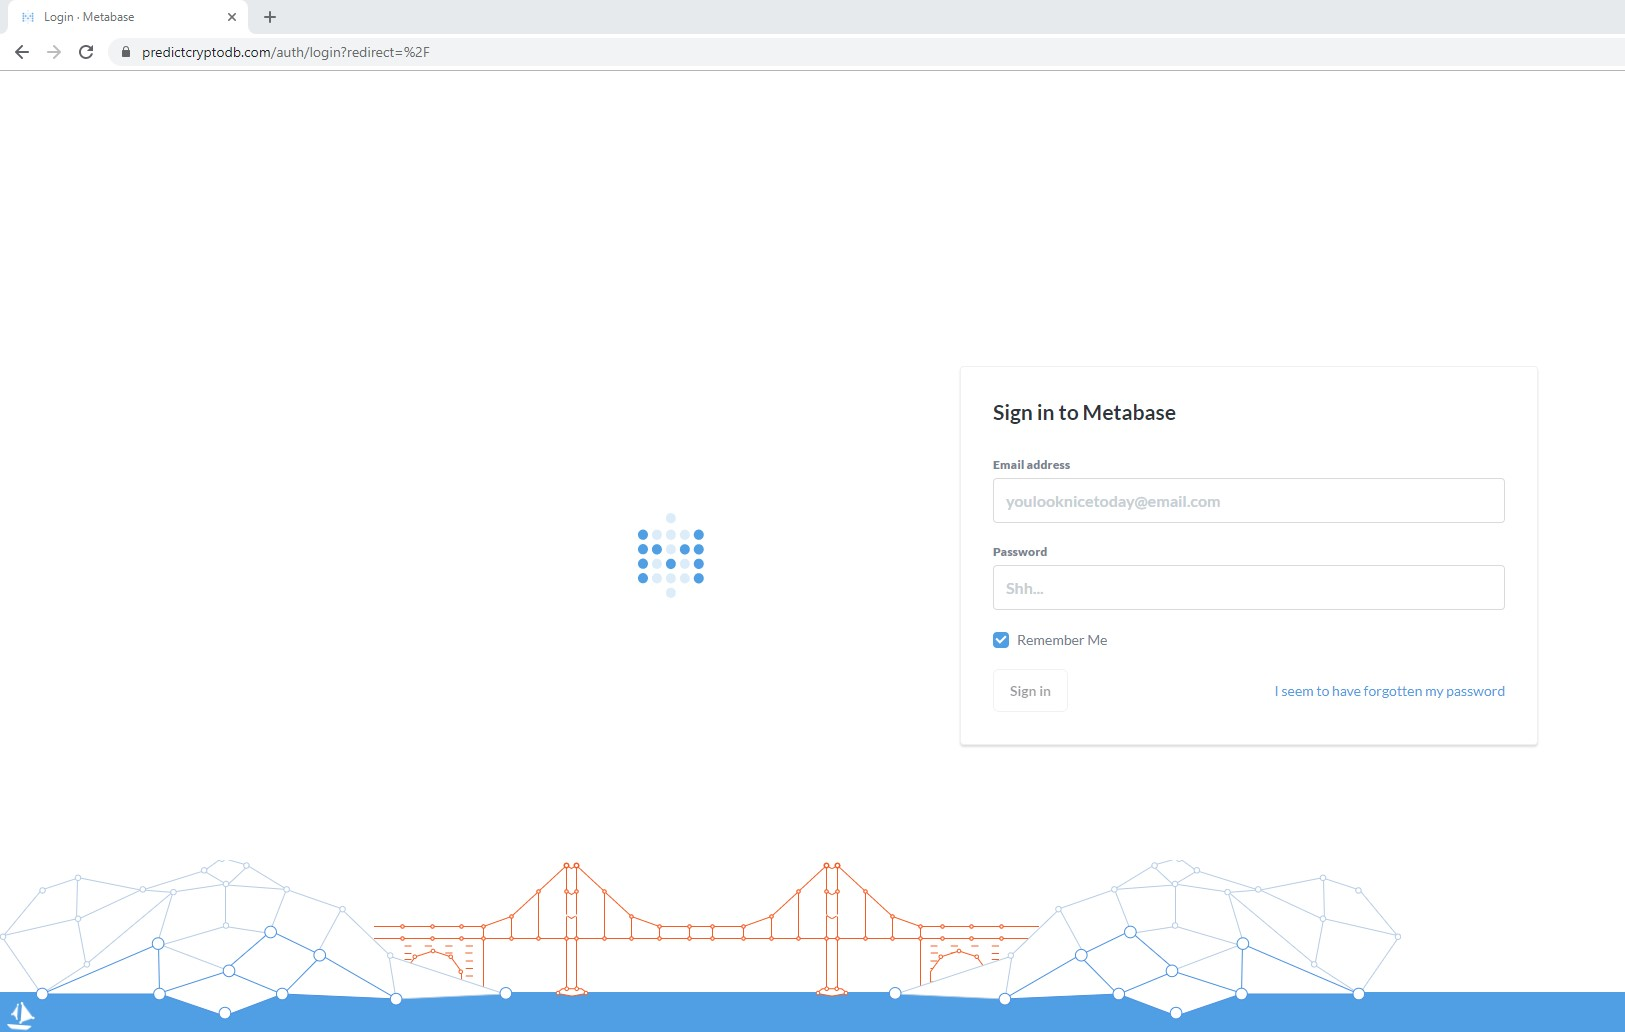
\includegraphics{images/MetabaseLogin.jpg}

  \begin{itemize}
  \item
    If you are having issues accessing the website, try spelling the url including \href{https://predictcryptodb.com}{\textbf{\emph{https://}}predictcryptodb.com}.
  \item
    Before you can login, you need to configure your account through the e-mail you should have received. If you did not receive the e-mail, check your spam folder first:

    \begin{figure}
    \centering
    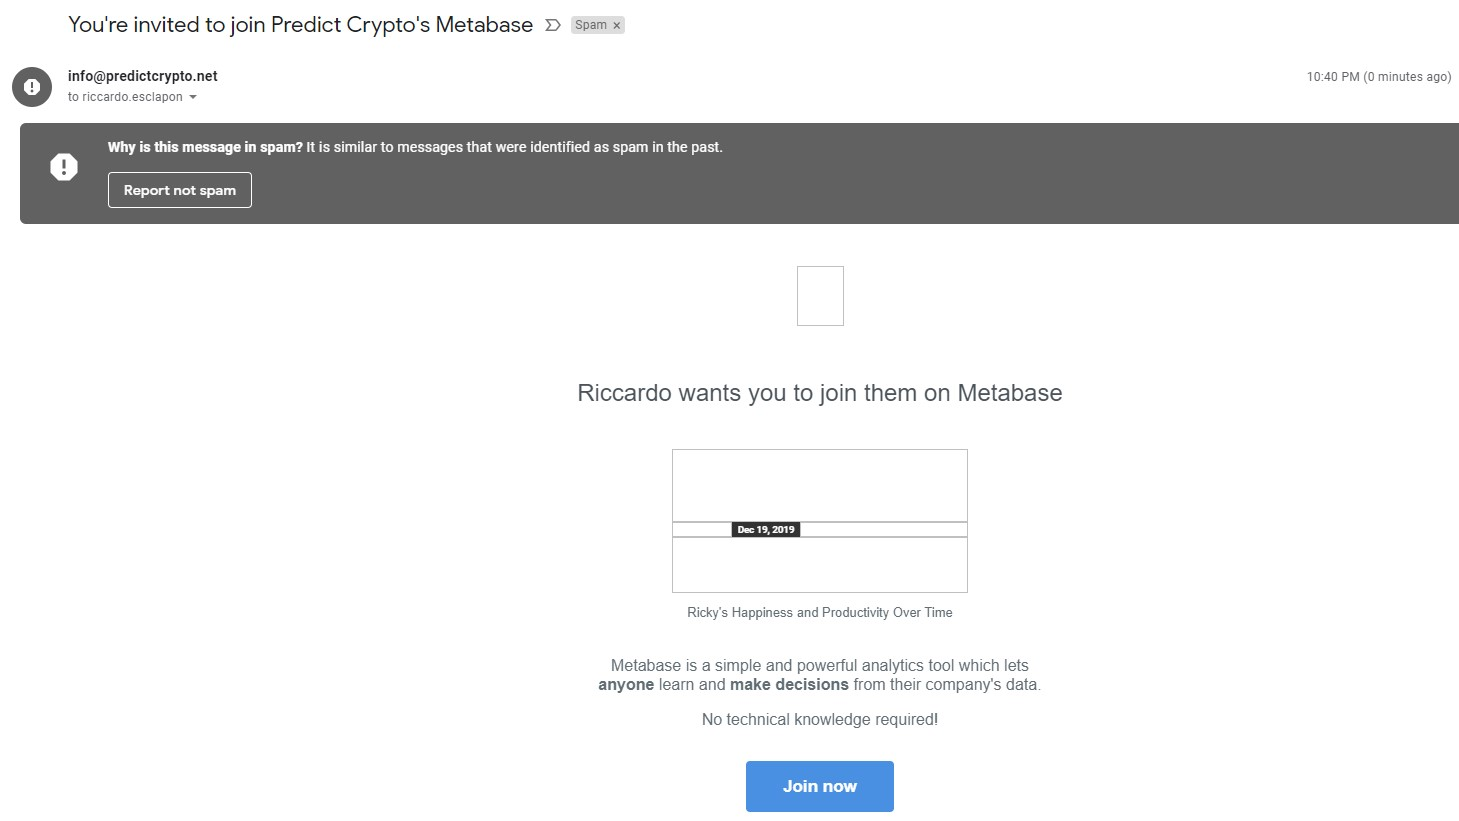
\includegraphics{images/MetabaseInvite.jpg}
    \caption{\emph{If you need the e-mail to setup your login, e-mail me}}
    \end{figure}

    \begin{itemize}
    \tightlist
    \item
      Configure your password and you will be able to use your e-mail and password to login in the future:
    \end{itemize}

    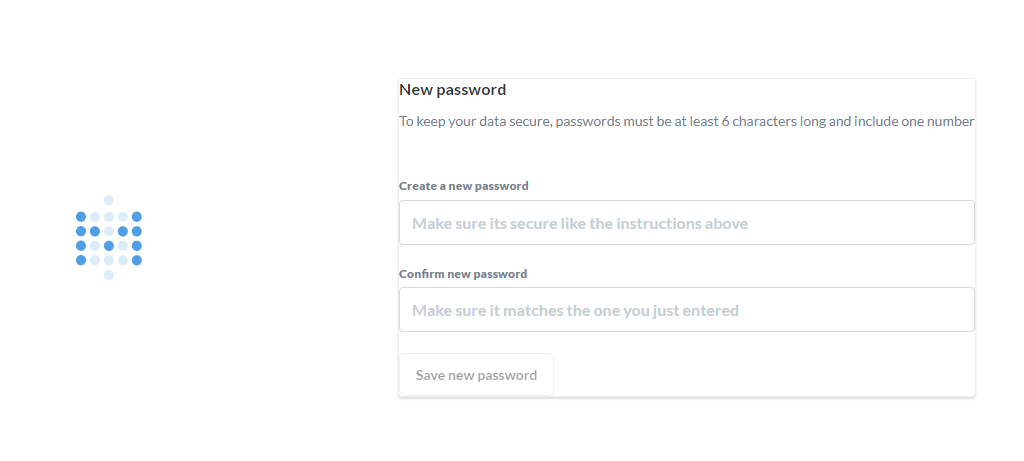
\includegraphics{images/MetabaseSetPassword.png}
  \end{itemize}
\item
  Once you have logged in, you should see a page that looks like this:

  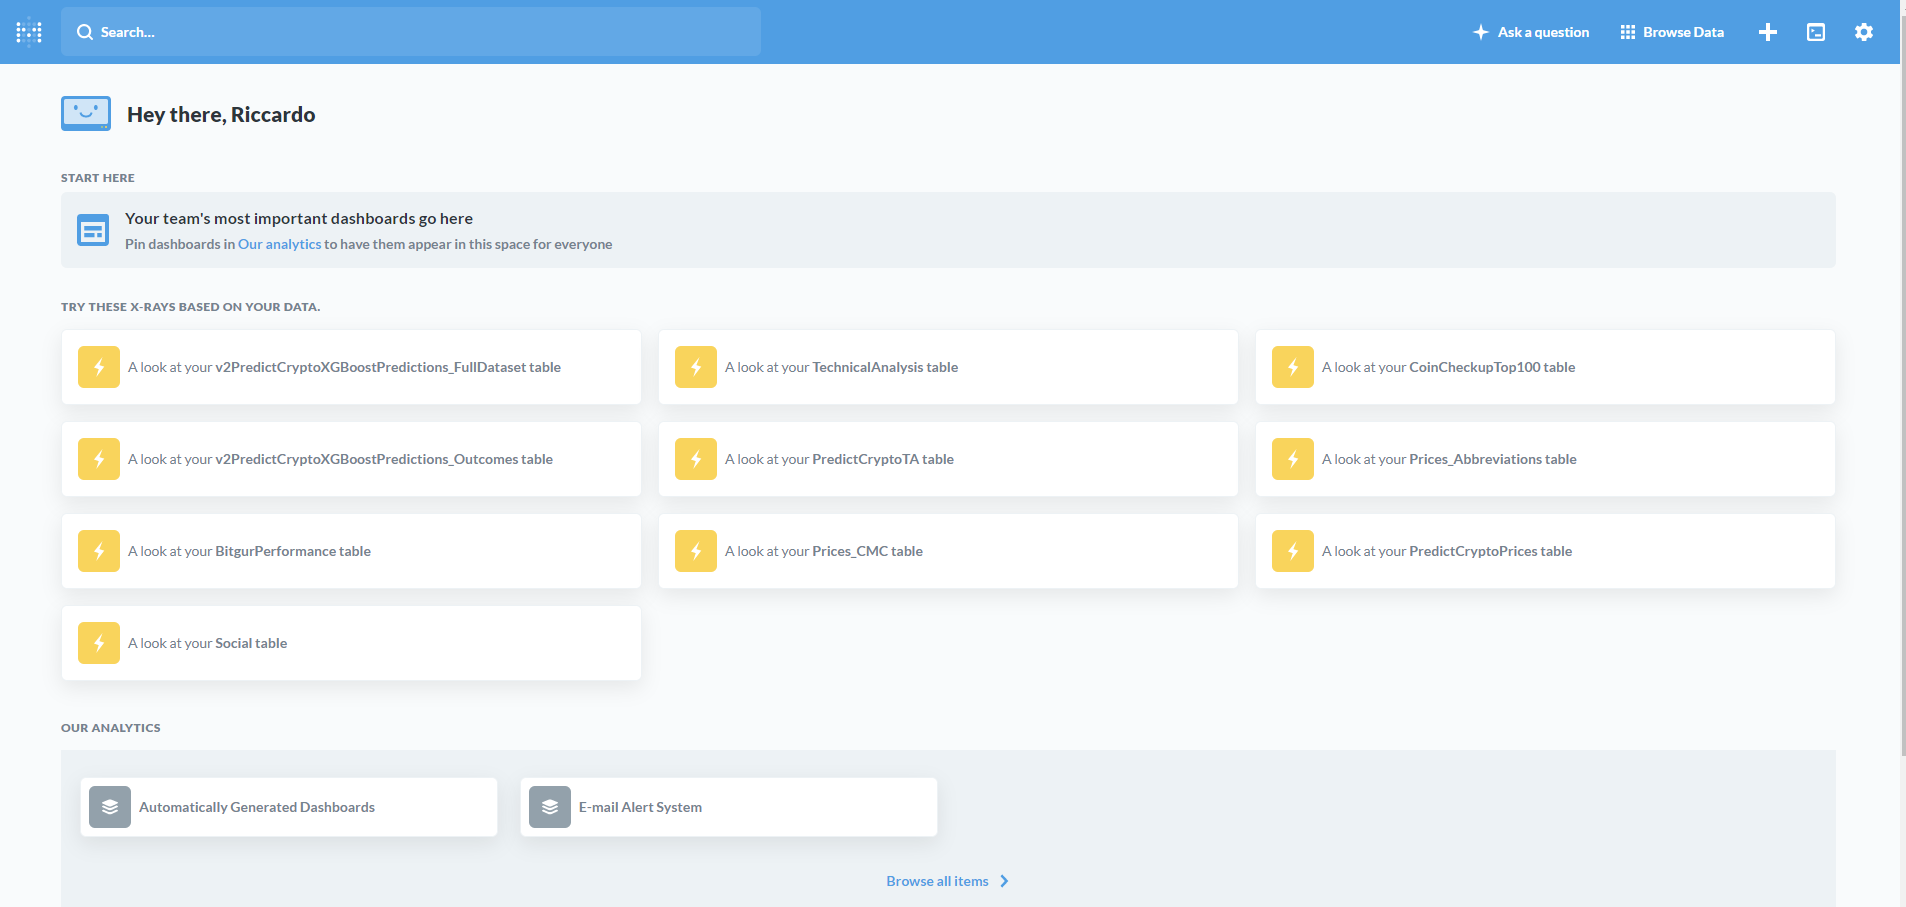
\includegraphics{images/MetabaseDashboard.png}
\end{enumerate}

In the next section we will talk about some good tables to get started on, and getting more comfortable navigating the layout of the website.

\hypertarget{useful-tables}{%
\chapter{Useful Tables}\label{useful-tables}}

\hypertarget{browse-data}{%
\section{Browse Data}\label{browse-data}}

Let's start by clicking on the \texttt{Browse\ Data} tab in the top right of the Metabase environment:

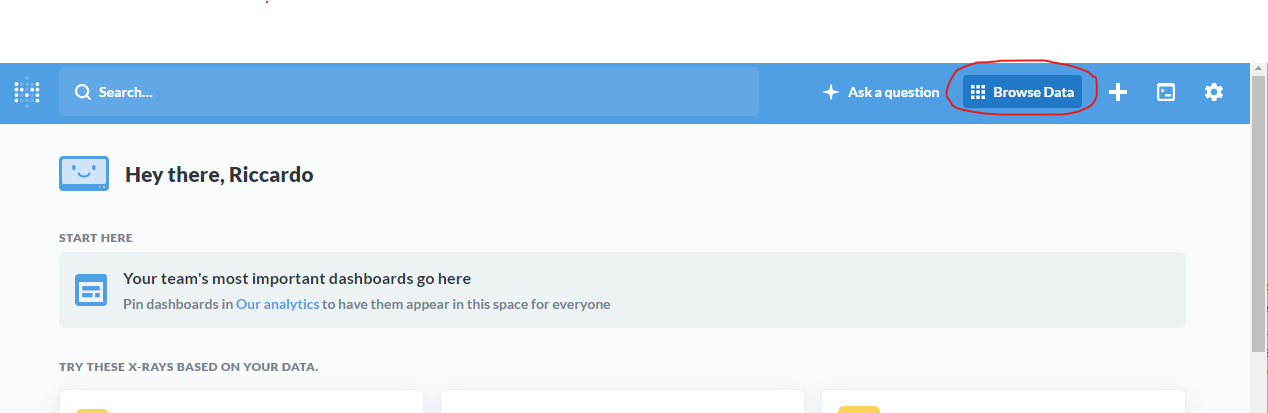
\includegraphics{images/MetabaseBrowseData.png}

Here, you will see two different options:

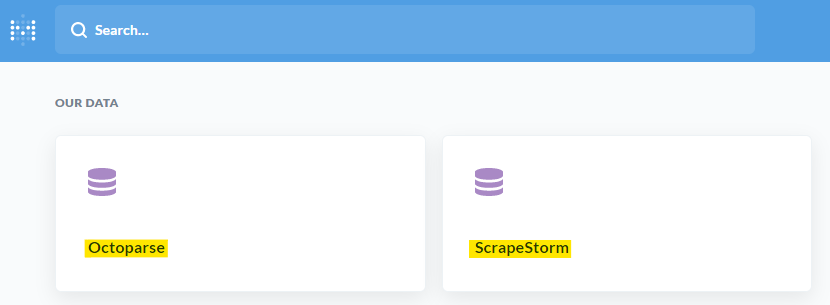
\includegraphics{images/DBSelection.png}

\begin{itemize}
\item
  \texttt{Octoparse} is the schema that is associated with data I have collected by using the \emph{Octoparse} web scraping software.
\item
  Conversely, \texttt{ScrapeStorm} is the schema associated with data collected using the \emph{ScrapeStorm} web scraping software.
\item
  Web scraping has its challenges in terms of stability, so I built some additional resilience by using two different tools that work independently of each other and do similar things (and in some cases collect the same data). Although not a perfect solution, having both up and running means we can usually fill the gaps that might arise in each tool respectively.

  \begin{itemize}
  \item
    The web scrapers that are run through Octoparse run on their servers in the cloud, which are very stable but have had some issues here and there in the past.
  \item
    The web scrapers that are run through ScrapeStorm run on a local machine on my end. I have a computer in the cloud that runs 24/7 but even after upgrading the hardware on it ScrapeStorm kept crashing, so this currently runs on my powerful desktop computer that is always on at home. When these run, the data flows in almost immediately, meaning if it's 4:05PM and you pulled the latest hour of data (which would be equivalent to the \texttt{max(***pkDummy***)}, more to come on that later on)
  \end{itemize}
\item
  Here is the size in MB of both the \texttt{Octoparse} database and the \texttt{ScrapeStorm} db as of the last time this document was refreshed (updated daily):
  \includegraphics{WebScrapingGuide_files/figure-latex/showTableSummary-1.pdf}
\end{itemize}

\textbf{Back in MetaBase, let's click on the option that says \texttt{Octoparse}:}

\begin{figure}
\centering
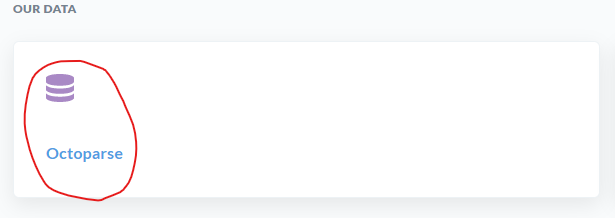
\includegraphics{images/OctoparseClick.png}
\caption{I would recommend starting here because this was the first/original database and will have more historical data compared to ScrapeStorm, which I got up and running much later}
\end{figure}

Now you should see the tables that are contained within the \texttt{Octoparse} schema. By hovering over each table, you will see three options appear, which will be better explained in the \protect\hyperlink{documentation-usage}{next section about \emph{Documentation Usage}}. In the screenshot the mouse is hovering over the \texttt{i} symbol for the Bitgur table:

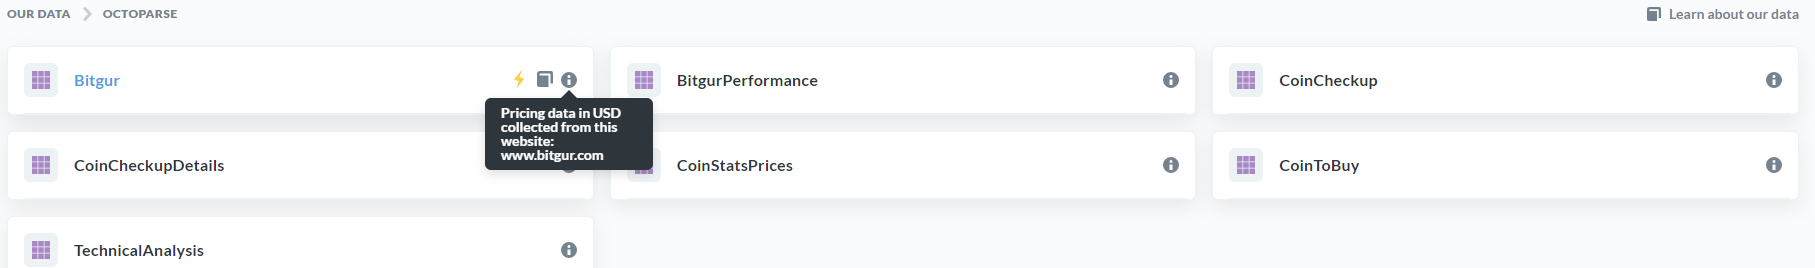
\includegraphics{images/OctoparseTableOptionsHover.png}

For now, let's go ahead and click on the name of the table \texttt{Bitgur}:


\includegraphics{images/BitgurTableSelect.png}

After clicking on the table name, you should see some example data show up. This shows the first 2,000 rows of data found in the table:

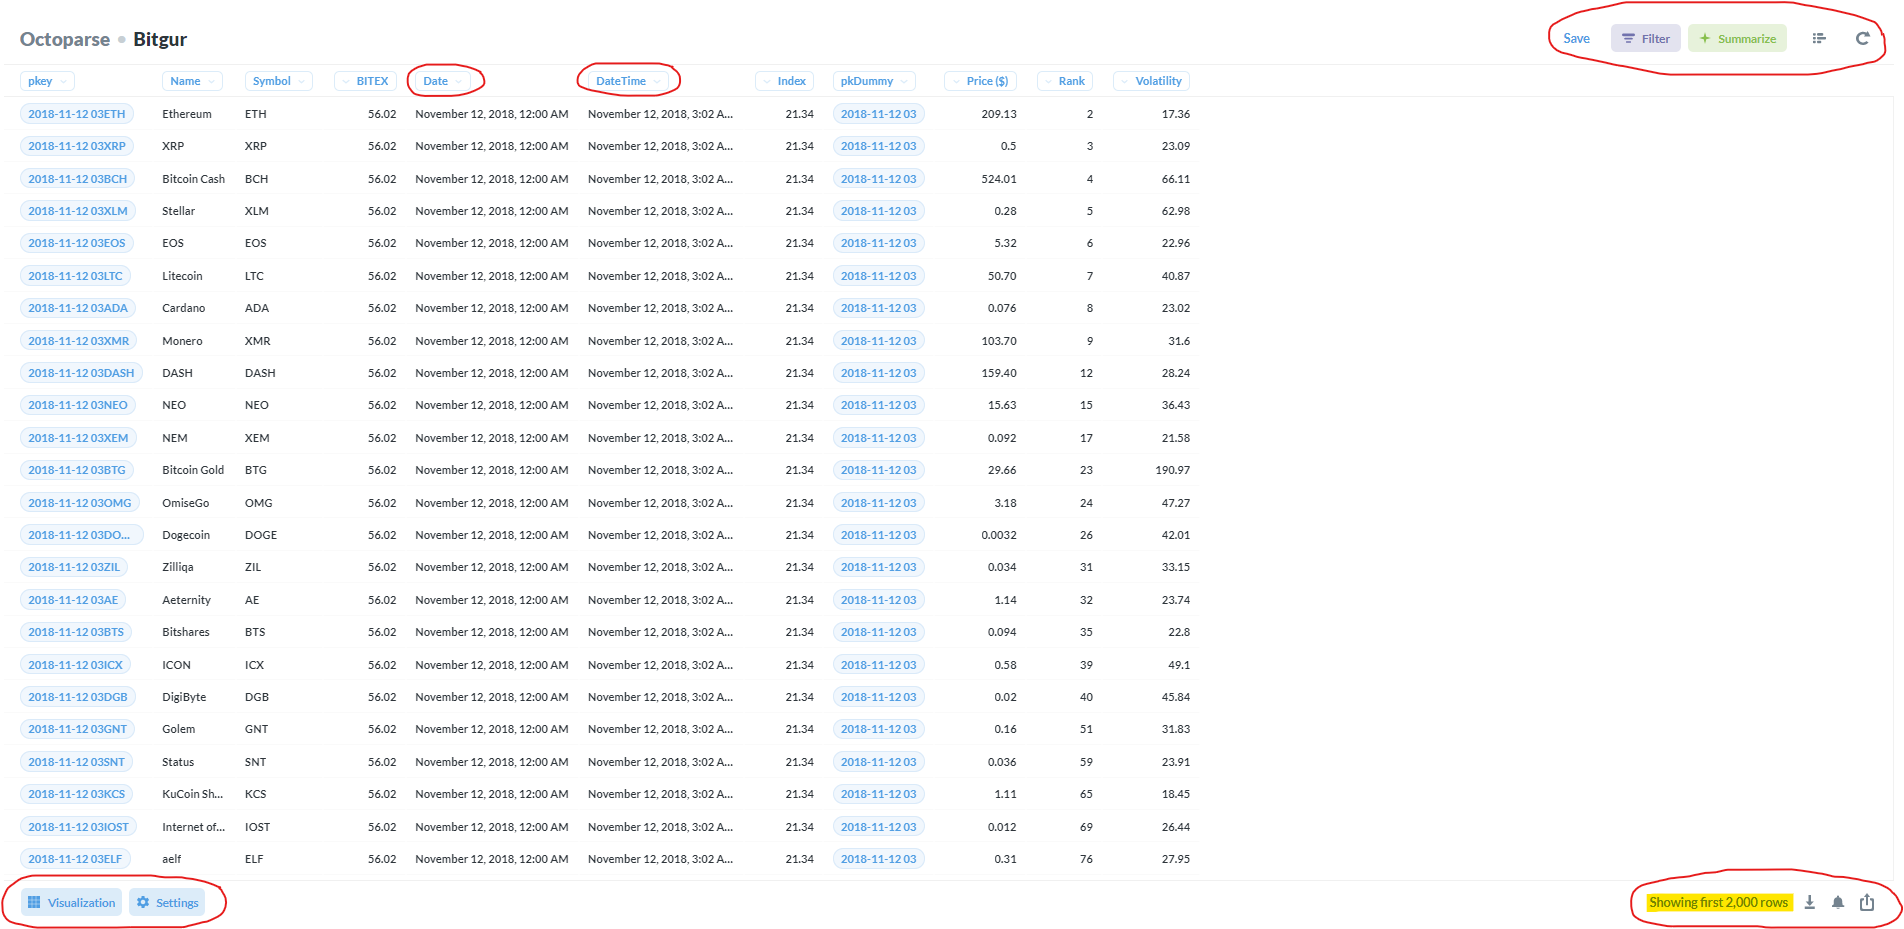
\includegraphics{images/BitgurPreview.png}

In the next section we will walk through some of the functionality associated with the things circled in red in the screenshot above using the Bitgur table as an example.

\hypertarget{useful-tables-1}{%
\section{Useful tables}\label{useful-tables-1}}

For the previews below, keep an eye out for a button to show more columns:
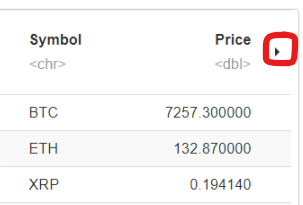
\includegraphics{images/MoreColumns.png}

\hypertarget{tables-in-octoparse-db}{%
\subsection{\texorpdfstring{Tables in \texttt{Octoparse} db}{Tables in Octoparse db}}\label{tables-in-octoparse-db}}

\hypertarget{bitgur}{%
\subsubsection{\texorpdfstring{\href{https://predictcryptodb.com/question/6}{\textbf{\texttt{Bitgur}}}}{Bitgur}}\label{bitgur}}

\begin{itemize}
\item
  Source: \url{https://bitgur.com/}
\item
  Data collected since: 2018-11-11
\end{itemize}

\hypertarget{bitgurperformance}{%
\subsubsection{\texorpdfstring{\href{https://predictcryptodb.com/question/7}{\textbf{\texttt{BitgurPerformance}}}}{BitgurPerformance}}\label{bitgurperformance}}

\begin{itemize}
\item
  This table is very similar to the \texttt{Bitgur} table, but this one includes some fields that summarize the short-term performance of the cryptocurrency in the short-term relative to when the data was collected.
\item
  The normal \texttt{Bitgur} table would have the prices fields, but not information about the performance over the previous 1h, 3h, etc..
\item
  Source: \url{https://bitgur.com/performance}
\item
  Data collected since: 2019-11-05
\end{itemize}

\hypertarget{add-more-tables}{%
\subsubsection{ADD MORE TABLES}\label{add-more-tables}}

\hypertarget{tables-in-scrapestorm-db}{%
\subsection{\texorpdfstring{Tables in \texttt{ScrapeStorm} db}{Tables in ScrapeStorm db}}\label{tables-in-scrapestorm-db}}

\hypertarget{scrapestorm.shrimpyprices}{%
\subsubsection{\texorpdfstring{\href{https://predictcryptodb.com/question/8}{\textbf{\texttt{ScrapeStorm.ShrimpyPrices}}}}{ScrapeStorm.ShrimpyPrices}}\label{scrapestorm.shrimpyprices}}

When using data from a table like the \texttt{BitgurPerformance}, the data is aggregared at a global level. Meaning, the Bitgur website connects to a certain number of exchanges, and calculates things like the overall Market Capitalization (\$), the 24h volume, etc. When it comes to the price, the website will average things across exchanges to get to the current price, which makes sense, but in my experience this is not as precise as it needs to be in order to programmatically trade on the cryptocurrency markets.

\begin{verbatim}
+ Therefore, a better approach is to collect the prices directly through the individual exchanges. Because I setup my trading system to work through a service called **Shrimpy**, I have been collecting prices for each exchange as reported through the Shrimpy website. This for example would be the page for the KuCoin exchange prices:
\end{verbatim}

\begin{itemize}
\item
  Source: \url{https://www.shrimpy.io/exchange}

  \begin{figure}
  \centering
  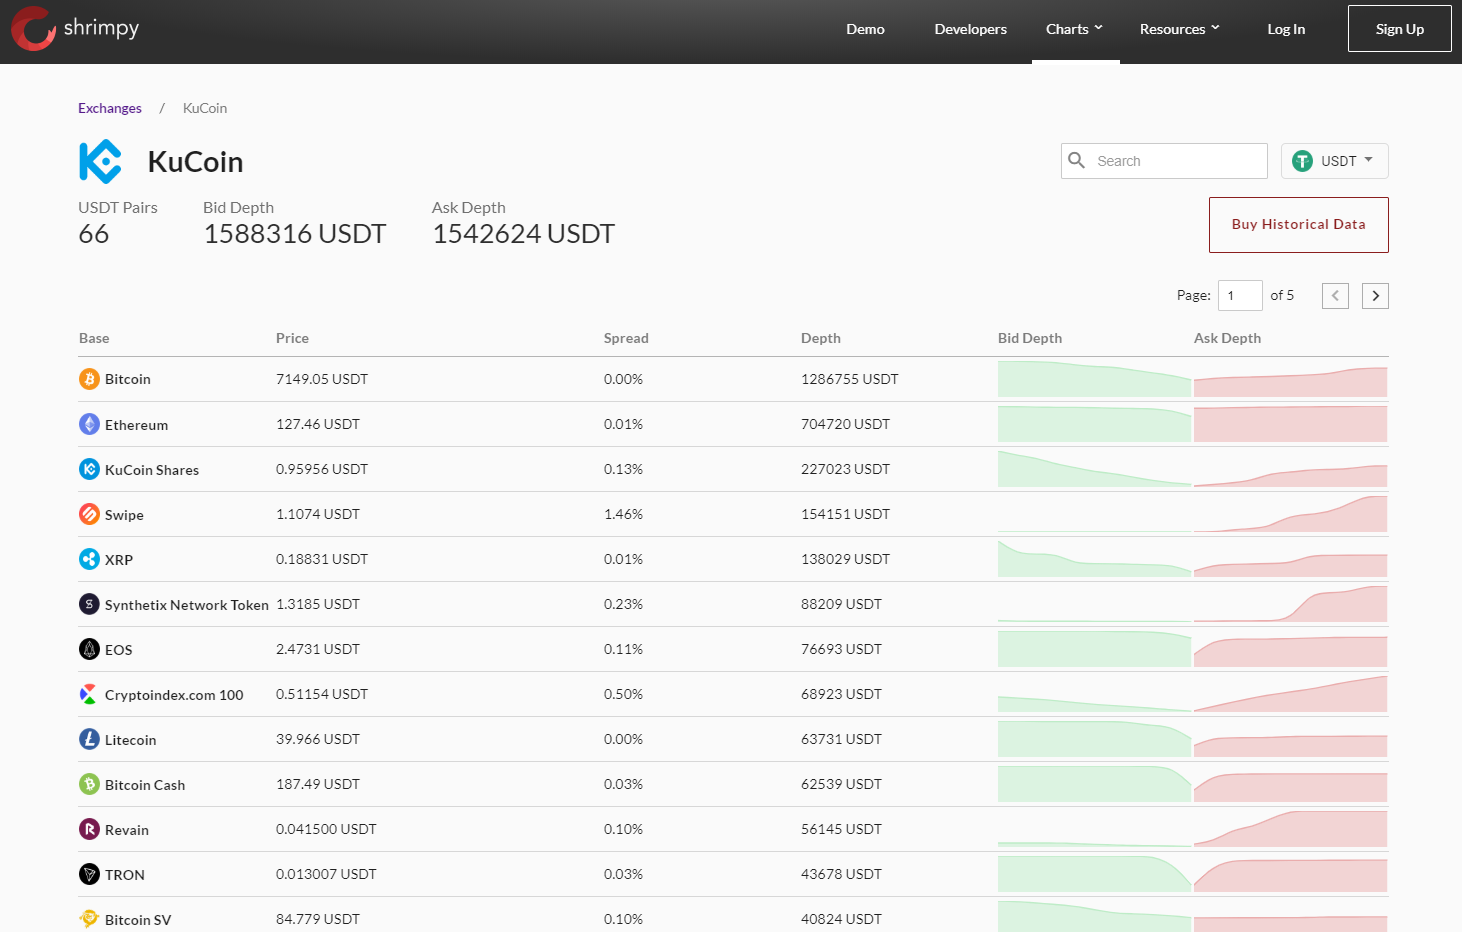
\includegraphics{images/ShrimpyKucoin.png}
  \caption{Example for the KuCoin exchange}
  \end{figure}
\end{itemize}

\hypertarget{scrapesstorm.shrimpypricesbtc}{%
\subsubsection{\texorpdfstring{\href{https://predictcryptodb.com/question/9}{\textbf{\texttt{ScrapesStorm.ShrimpyPricesBTC}}}}{ScrapesStorm.ShrimpyPricesBTC}}\label{scrapesstorm.shrimpypricesbtc}}

This table is exactly like the previous one \texttt{ShrimpyPrices}, but this one shows prices in BTC instead of being in USD

\hypertarget{number-of-rows-by-table}{%
\subsection{Number of rows by table}\label{number-of-rows-by-table}}

\begin{tabular}{l|l|r}
\hline
Database & Table Name & Rows\\
\hline
ScrapeStorm & ShrimpyPricesBTC & 570220\\
\hline
ScrapeStorm & Messari-2019-09-26 & 829532\\
\hline
ScrapeStorm & BitgurBasic & 450889\\
\hline
ScrapeStorm & ShrimpyPrices & 299491\\
\hline
ScrapeStorm & KuCoinPrices & 38820\\
\hline
ScrapeStorm & Symbols & 817056\\
\hline
Octoparse & v2PredictCryptoXGBoostPredictions\_Outcomes & 14135169\\
\hline
Octoparse & BitgurPerformance & 3030001\\
\hline
Octoparse & Bitgur & 23138495\\
\hline
Octoparse & TechnicalAnalysis & 2191923\\
\hline
Octoparse & CoinCheckupTop100 & 681092\\
\hline
Octoparse & AYX191231dabf06dfe9758fb1a5477 & 17764\\
\hline
Octoparse & v2PredictCryptoXGBoostPredictions & 54262\\
\hline
Octoparse & v2PredictCryptoXGBoostPredictions\_FullDataset & 54414\\
\hline
\end{tabular}

\hypertarget{usage-guide}{%
\chapter{Usage Guide}\label{usage-guide}}

\hypertarget{pulling-most-recent-data}{%
\section{Pulling Most Recent Data}\label{pulling-most-recent-data}}

Let's say you went ahead and trained a predictive model using the data found in the database and now you want to test making some \emph{semi-live} predictions, how would you go about pulling the latest data to make predictions on?

\begin{itemize}
\item
  pkDummy
\item
  pkey
\end{itemize}

Make a note that can't do this between different schemas because the Octoparse one is in UTC and the ScrapeStorm one in local time. Only real effective way I found do to that is through Alteryx tools.

\hypertarget{data-exploration}{%
\section{Data Exploration}\label{data-exploration}}

Let's explore some of the functionality found in Metabase using the \texttt{Bitgur} table results page we got to at the end of the previous section.

\begin{itemize}
\item
  The first thing I want to point out, is that you can click on each field to open a menu with an assortment of options based on the data type. For example, if we click on the \textbf{Price} field, these are the options we are given:

  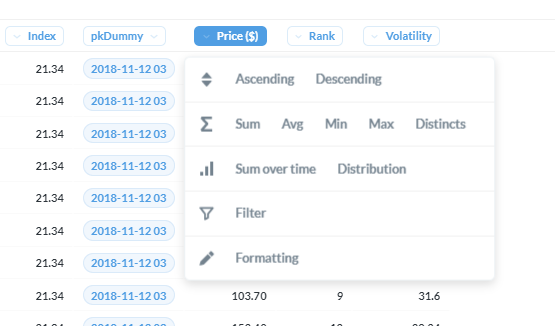
\includegraphics{images/PriceFieldOptions.png}

  \begin{itemize}
  \item
    The Date field is a different data types and offers different options. For example we could sort the data by the \textbf{Date} field \textbf{Descending}:

    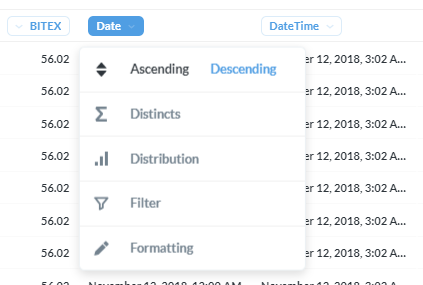
\includegraphics{images/DateDescendingOption.png}

    \begin{itemize}
    \item
      Which would return the first 2,000 rows again but this time sorted showing the largest values first (meaning the latest date):

      \begin{figure}
      \centering
      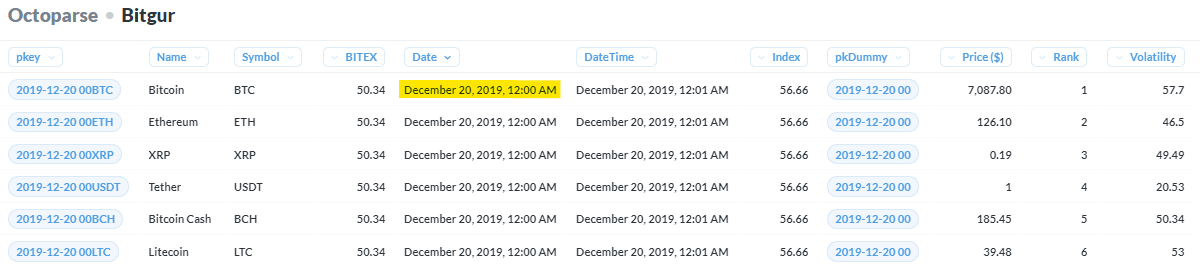
\includegraphics{images/DateDescendingOutcome.png}
      \caption{If the \texttt{Bitgur} table is not being very responsive, try using the \texttt{BitgurPerformance} table instead, which should load faster (but has less historical data, this table is described in \protect\hyperlink{some-other-useful-tables}{a section below})}
      \end{figure}
    \end{itemize}
  \end{itemize}
\item
  Next, let's click on the purple \texttt{Filter} button in the top right of the page:

  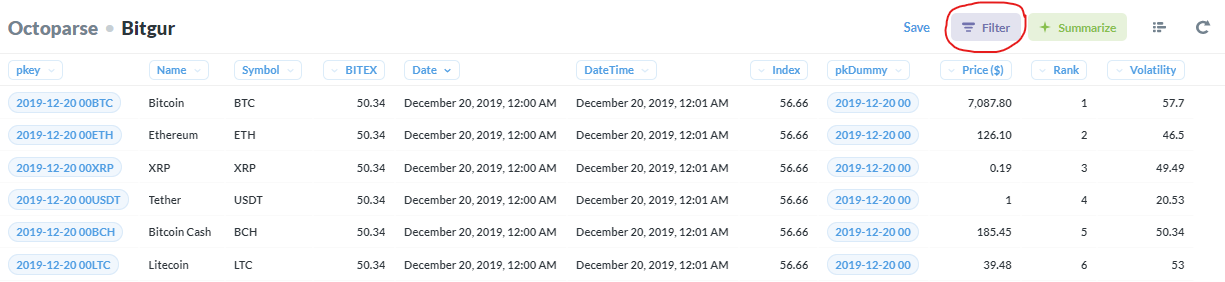
\includegraphics{images/FilterButton.png}

  \begin{itemize}
  \item
    Now you should see the following sidebar pop-up:

    \begin{figure}
    \centering
    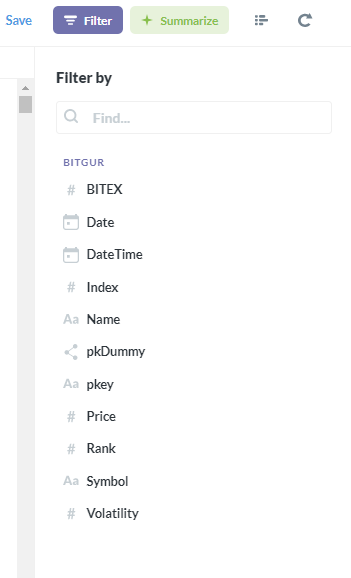
\includegraphics{images/FilterSidebar.png}
    \caption{Notice how the icons next to the field names correspond to their data types}
    \end{figure}

    \begin{itemize}
    \item
      Let's do a quick example filtering based on the \textbf{DateTime} field:

      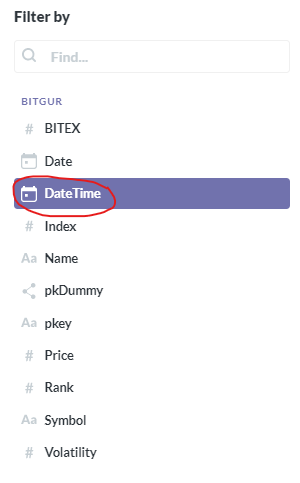
\includegraphics{images/DateTimeClick.png}

      \begin{itemize}
      \tightlist
      \item
        Let's add a filter to only select data where the \textbf{DateTime} field is from the last 7 days:
      \end{itemize}

      \begin{figure}
      \centering
      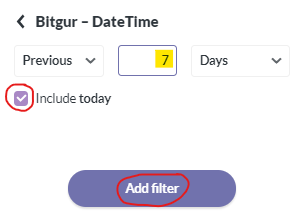
\includegraphics{images/DateTimeOptions.png}
      \caption{\emph{please be patient as this loads or do the same with a different table that contains less historical data}}
      \end{figure}
    \end{itemize}
  \end{itemize}
\item
  Now that we have filtered the data down to the subset we are interested in, let's adjust the look of the table using the \texttt{Settings} option in the bottom left:

  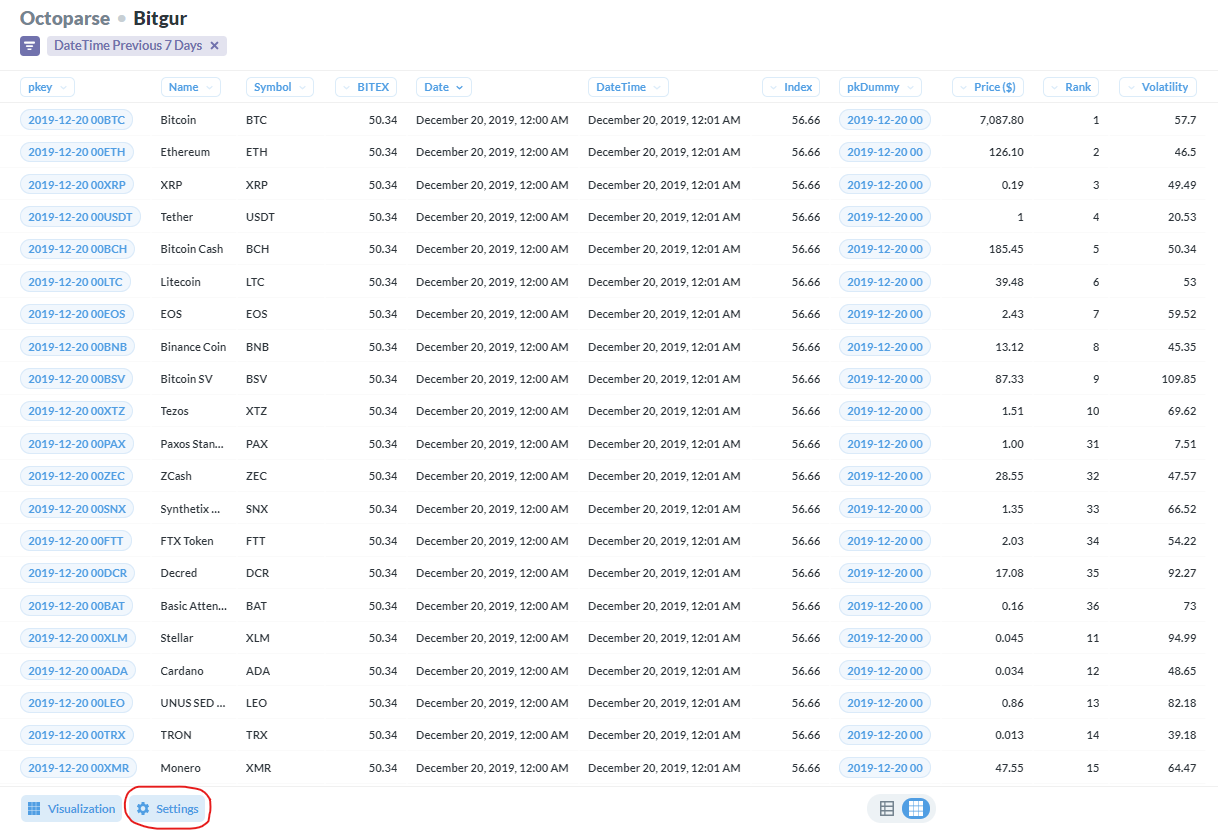
\includegraphics{images/BitgurTableSettings.png}

  \begin{itemize}
  \item
    After clicking on the \texttt{Settings} button, you should see a sidebar show up on the left. First, let's edit the settings for the \textbf{Price} field:

    
\includegraphics{images/BitgurPriceSettings.png}

    \begin{itemize}
    \item
      And let's set the currency to be displayed with every cell instead of in parenthesis in the column name:

      
\includegraphics{images/PriceShowCurrency.png}

      \begin{itemize}
      \tightlist
      \item
        Now the currency field will look like this for each row:
      \end{itemize}

      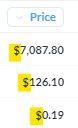
\includegraphics{images/BitgurPriceModified.png}
    \end{itemize}
  \item
    Let's also do a quick edit to the \textbf{Volatility} field settings:

    
\includegraphics{images/BitgurVolatilitySettings.png}

    \begin{itemize}
    \tightlist
    \item
      Enable the setting to \texttt{Show\ a\ mini\ bar\ chart}:
    \end{itemize}

    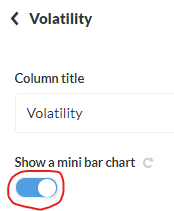
\includegraphics{images/ShowMiniBarChart.png}

    \begin{itemize}
    \item
      Now each row should have a bar that is filled based on the current value compared to the minimum and maximum values for that field for the current subset of the data:

      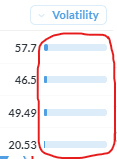
\includegraphics{images/VolatilityMiniBarChart.png}

      \begin{itemize}
      \tightlist
      \item
        If we sort the data by \textbf{Volatility} in \emph{descending} order, we can see the row that sets the bar for the maximum for the rest of the rows:
      \end{itemize}

      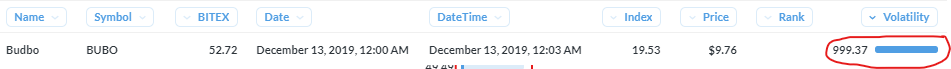
\includegraphics{images/MaximumVolatility.png}
    \item
      Now let's also add some conditional formatting to the \textbf{Volatility} field, which will color each row when a certain criteria is met. Go back to the \texttt{Settings} page of the table, and this time click on \texttt{Conditional\ Formatting}:

      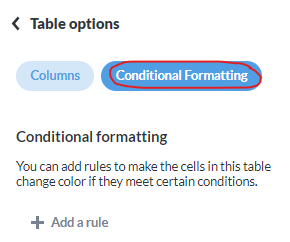
\includegraphics{images/ConditionalFormattingSelect.png}

      \begin{itemize}
      \tightlist
      \item
        Now we can create a rule to highlight rows with a value for \textbf{Volatility \textgreater{} 50}:
      \end{itemize}

      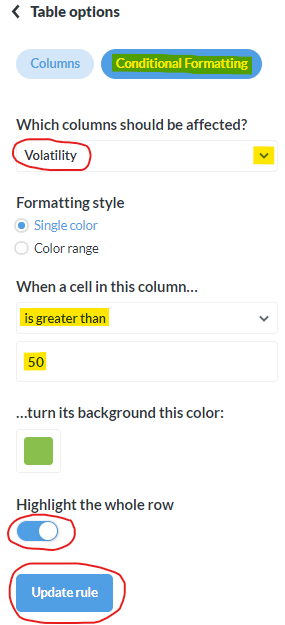
\includegraphics{images/ConditionalFormattingRule.png}

      \begin{itemize}
      \tightlist
      \item
        The table's rows should now be highlighted when the criteria is met:
      \end{itemize}

      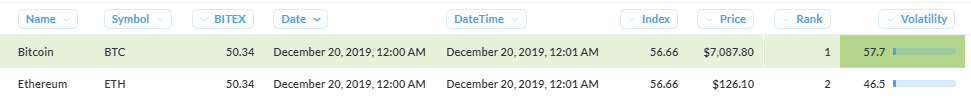
\includegraphics{images/ConditionalFormattingOutput.png}
    \end{itemize}
  \end{itemize}
\end{itemize}

\hypertarget{exporting-data}{%
\subsection{Exporting Data}\label{exporting-data}}

(make a note about confidentiality of the data)

\hypertarget{answer-questions}{%
\section{Answer Questions}\label{answer-questions}}

\hypertarget{creating-dashboards}{%
\section{Creating dashboards}\label{creating-dashboards}}

\hypertarget{documentation-usage}{%
\chapter{Documentation Usage}\label{documentation-usage}}

Everything you have visibility to within the Metabase environment is documented. Meaning, every table you see has a description which includes the URL of where the data is collected (as well as the web scraping methodology where informative), and every field within those tables has also been documented on \href{https://predictcryptodb.com}{predictcryptodb.com}. Every table you have visibility to also has an e-mail alert system that alerts me if the data stops flowing through on an hourly (or daily for some) basis. If anything becomes broken I will remove the visibility of that table within Metabase, so if a table is found within the Metabase environment you can assume the web scraper for that table is still functioning correctly and that the data is uploaded to the table on an automated schedule. I think Metabase could do a better job at making the documentation for the different tables more intutitive to find, so hopefully this guide can provide some clarity where Metabase might be lacking.

\hypertarget{pkdummy-and-pkey}{%
\section{pkDummy and pkey}\label{pkdummy-and-pkey}}

\hypertarget{navigating-the-metabase-interface}{%
\section{Navigating the Metabase interface}\label{navigating-the-metabase-interface}}

\hypertarget{using-x-rays-to-explore-a-table}{%
\section{Using x-rays to explore a table}\label{using-x-rays-to-explore-a-table}}

\begin{itemize}
\tightlist
\item
  caveat that the database doesn't have the greatest resources that a big company would be able to provide and how this database costs around \$220 a month to maintain vs.~what a company would spend
\end{itemize}

(could really use a section on explaining the way pkDummy, pkey work and how they follow two different time zones, show Alteryx trick to deal with the trickiness of UTC not having daylight savings and our local times having it)

\hypertarget{additional-tips}{%
\chapter{Additional Tips}\label{additional-tips}}

\hypertarget{creating-variables-for-queries}{%
\section{Creating Variables for queries}\label{creating-variables-for-queries}}

\begin{itemize}
\item
  Within new question, click on the ``x'' symbol to open sidebar on the side and learn how to use variables:

  \begin{itemize}
  \tightlist
  \item
    \{\{variable\_name\}\} creates a variable in this SQL template called ``variable\_name''. Variables can be given types in the side panel, which changes their behavior. All variable types other than ``Field Filter'' will automatically cause a filter widget to be placed on this question; with Field Filters, this is optional. When this filter widget is filled in, that value replaces the variable in the SQL template.
  \end{itemize}
\end{itemize}

\hypertarget{embedding-anything-created-on-metabase}{%
\section{Embedding anything created on Metabase}\label{embedding-anything-created-on-metabase}}

\hypertarget{creating-e-mail-triggers}{%
\section{Creating e-mail triggers}\label{creating-e-mail-triggers}}

\hypertarget{pulses}{%
\subsection{Pulses}\label{pulses}}

\hypertarget{using-the-shrimpy-python-library}{%
\section{Using the Shrimpy-Python Library}\label{using-the-shrimpy-python-library}}

This section is a bit more \emph{expert level} and I don't really expect anyone to go down this route, but I figured it was worth having a small section on using the Shrimpy software for trading cryptocurrencies by using their Python package. This is a particularly good way to execute trades on the cryptocurrency markets because rather than having to connect to and manage each API individually, you can connect up to 16 exchanges to your Shrimpy account and programmatically trade on every one of them using the same set of functions in Python.

\begin{verbatim}
## Warning: Closing open result sets
\end{verbatim}

\begin{verbatim}
## [1] TRUE
\end{verbatim}

\bibliography{book.bib,packages.bib}


\end{document}
